\documentclass[10pt,a4paper]{article}
\usepackage[utf8]{inputenc}
\usepackage[english]{babel}
\usepackage{graphicx}
\usepackage{pdfpages}
\usepackage[top=1in, bottom=1.25in, left=1.25in, right=1.25in]{geometry}
\usepackage{comment}
\usepackage{float}
\usepackage{cite}
\usepackage{hyperref}


\author{Kevin}
\title{NoName TFG}
\date{2019-02-05}

\graphicspath{{images/}}
\makeindex

%No ident first line
\setlength\parindent{0pt}

\begin{document}
	\pagenumbering{gobble}
	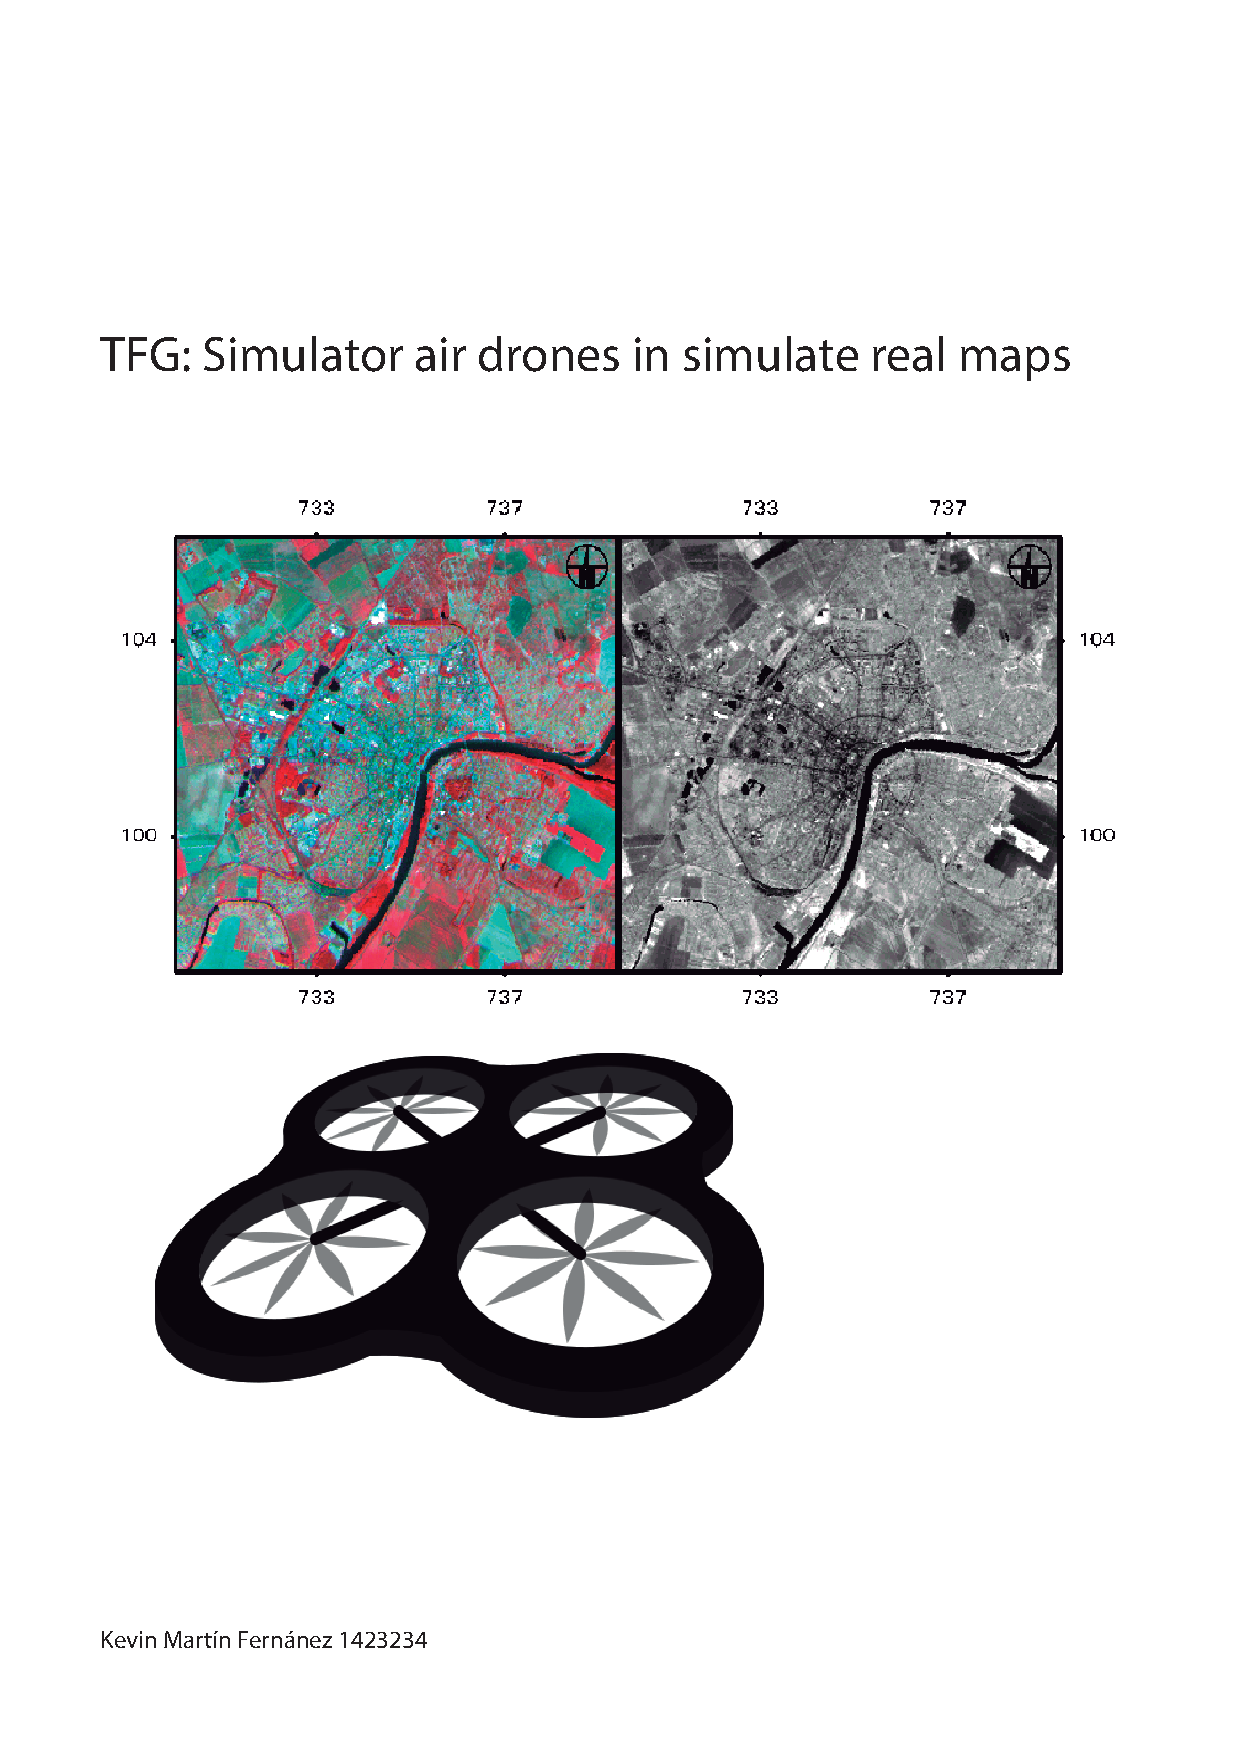
\includepdf{PortadaTFG}
	\tableofcontents
	\newpage
	\listoffigures
	%\listoftables

	\newpage
	\pagenumbering{arabic}
	\section{Introduction}
	It's a try
	\subsection{Objective}
	
	\subsection{State of the art}
	In this section we will analyse the different applications exists for a similar objectives, in this way we will decide from what point we start to work and what is the actual situation of the simulators tools for analyze real terrains and capture pictures to use on deep learning algorithms.
	
	\subsubsection{Carla CV}
	Carla CV \cite{CarlaCV} is a realistic car simulator made on Unreal Engine, the utility of this is generate synthetic images to train neural networks that allow drive a autonomous car in a safe way without endangering pedestrians.

	\begin{figure}[h!]
		\centering
		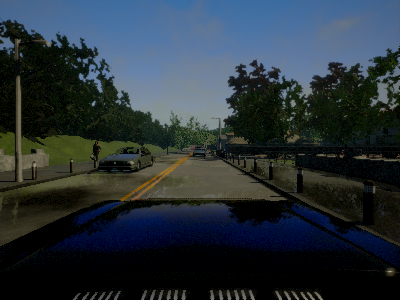
\includegraphics[height=8cm]{carla_img}
		\caption{Carla on-board RGB camera on car}
		\label{figure:carlargb}
	\end{figure}
	
	In the demo we can see a synthetic environment where can drive a car, this car is possible of drive through a python script, and allow record different cameras as we can see in the figure \ref{figure:carlargb} and apply different types of view how can they be RGB, depth or segmentation. 

	%TODO Explicar la forma en la que se comunica python y unreal
	
	\newpage
	\subsubsection{AirSim (Microsoft)}	
	AirSim \cite{AirSim} is a simulator for drones and cars, built on Unreal Engine. This utility is compatible with popular flight controllers, xbox controller and python scripting. We can visualize different cameras as we can see in the figure \ref{figure:airsim}  

	\begin{figure}[h!]
		\centering
		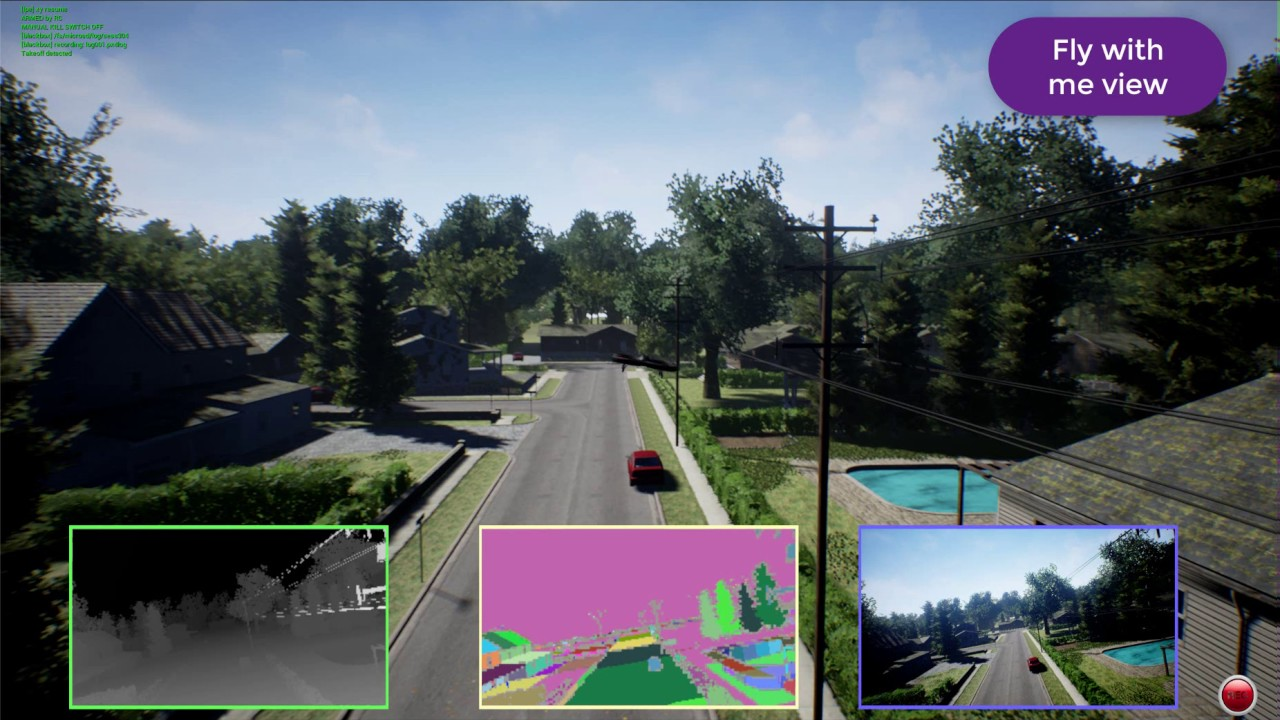
\includegraphics[height=8cm]{airsim}
		\caption{AirSim simulator screenshot}
		\label{figure:airsim}
	\end{figure}

	\subsubsection{Conclusions}
	Until now they have done diferents simulators for generate synthetic images with the objective of generate data to train diferents algorithm of deep learning, we has drone and car simulators to navigate in a map with cameras onboard that they have incorporated differents views how can they be RGB, depth or segmentation. Therefore, we can consider as base use the modules:
	\begin{itemize}
	\item Drone simulator
	\item Segmentations
	\end{itemize}

	Also we see that not exists other software that incorporate real geographic data for the simulations. For that reason, not exists any refererence to considere as base of our project.

	\section{Project structure}

	\subsection{Python Scripts}
	\subsection{Unreal Engine Simulator}
	\subsection{Communication Python-Unreal}

	\section{Satellite Data}
	\subsection{Unreal Engine Import}

	\section{Conclusions}
		
\newpage
\bibliography{biblio}
\bibliographystyle{plain}
	
\end{document}